\documentclass[border=6pt]{standalone}
\usepackage{garamondx}
\usepackage{pgfplots}
\usepackage{tikz}
\usepgfplotslibrary{units}
\usepackage{xcolor}
\definecolor{redtea}{rgb}{0.6823529412,0.2792156863,0.2666666667}
\definecolor{darkolivegreen}{rgb}{0.33, 0.42, 0.18}
\definecolor{darkbyzantium}{rgb}{0.36, 0.4, 0.33}
\definecolor{darkelectricblue}{rgb}{0.33, 0.41, 0.47}
\definecolor{deepchestnut}{rgb}{0.73, 0.31, 0.6}
\definecolor{azuremist}{rgb}{0.94, 1.0, 1.0}
\usepackage{siunitx}
\usepackage{changepage}
\usepackage{calc}
\pgfplotsset{samples}



\begin{document}
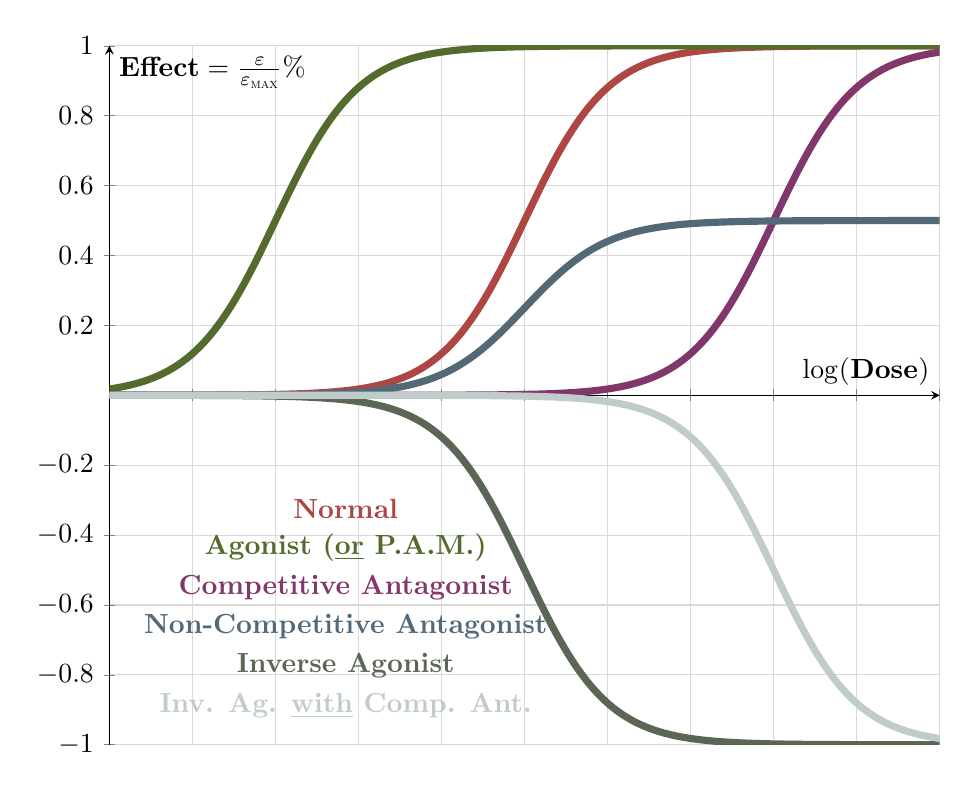
\begin{tikzpicture}
\begin{axis}[
width=\linewidth,
grid=major,
grid style={gray!30},
axis lines=middle,
xmax=10,
xmin=-0,
ymin=-1,
ymax=1,
xlabel={\scshape $\mathbf{\log}$(\textbf{Dose})},
ylabel={\scshape \textbf{Effect}$\;=\frac{\varepsilon}{\varepsilon_{\text{max}}}\%$},
xtick={},
xticklabels={}
]
\addplot[redtea] [line width=0.6ex,smooth,domain=-0:30,samples=1000] {1/(1+exp(-2*(x-5)))};%normal
\addplot[deepchestnut!70!black] [line width=0.6ex,smooth,domain=-0:30,samples=1000] {1/(1+exp(-2*(x-8)))};%comp ant
\addplot[darkolivegreen] [line width=0.6ex,smooth,domain=-0:30,samples=1000] {1/(1+exp(-2*(x-2)))};%agonist
\addplot[darkelectricblue] [line width=0.6ex,smooth,domain=-0:30,samples=1000] {0.5/(1+exp(-2*(x-5)))};%non comp ant
\addplot[darkbyzantium] [line width=0.6ex,smooth,domain=-0:30,samples=1000] {-(1/(1+exp(-2*(x-5))))};%inverse agonist
\addplot[azuremist!80!black] [line width=0.6ex,smooth,domain=-0:30,samples=1000] {-(1/(1+exp(-2*(x-8))))};%inverse + comp ant
\end{axis}

\node at(3,3) {\textcolor{redtea}{\scshape\bfseries Normal}};
\node at(3,2.5) {\textcolor{darkolivegreen}{\scshape\bfseries Agonist (\underline{or} P.A.M.)}};
\node at(3,2) {\textcolor{deepchestnut!70!black}{\scshape\bfseries Competitive Antagonist}};
\node at(3,1.5) {\textcolor{darkelectricblue}{\scshape\bfseries Non-Competitive Antagonist}};
\node at(3,1) {\textcolor{darkbyzantium}{\scshape\bfseries Inverse Agonist}};
\node at(3,0.5) {\textcolor{azuremist!80!black}{\scshape\bfseries Inv. Ag. \underline{with} Comp. Ant.}};
\end{tikzpicture}
\end{document}
